% Koma-Script Basisklasse
\documentclass[a4paper,12pt,pagesize,headsepline,bibtotoc,titlepage]{scrartcl}

% \usepackage[ngerman]{babel}		% deutsche Trennmuster
\usepackage[utf8]{inputenc}		% direkte Eingabe von Umlauten & Co. (Vorsicht: Encoding im Editor muss auch UTF-8 sein!)
\usepackage{comment}

\usepackage[T1]{fontenc}			% T1-Schriften

\usepackage{mathptmx}			% Times/Mathe \rmdefault
\usepackage[scaled=.90]{helvet}	% Skalierte Helvetica \sfdefault
\usepackage{courier}			% Courier \ttdefault

% Zusatzpakete für mehr mathematische Symbole, Einfügen von Grafiken
% und bessere Bildunterschriften
\usepackage{amsmath,amsthm,amsfonts,graphicx,caption}

% Wenn man direkt mit dem pdflatex eine PDF-Datei erzeugt, sollten diese beiden Pakete eingebunden werden
\usepackage{hyperref} % Hyperlinks anklickbar
\usepackage{ae,aecompl} % bessere Bildschirmschriftarten usw.
\usepackage{epstopdf} % support eps
\usepackage{xcolor}
\usepackage{wrapfig}
\usepackage{ulem}

\renewcommand{\emph}[1]{\textit{#1}}

\pagestyle{headings}

% Abstand der Kopfzeile vom Text:
\headsep4mm

\typearea[current]{current}     % Satzspiegel neu berechnen

% andere Bildunterschrift mit Hilfe von caption
\renewcommand{\figurename}{Fig.}  % Thomas: Voher "Abb."
\renewcommand{\captionlabelfont}{\bf}
\newcommand\todo[1]{\textbf{\textcolor{red}{#1}}}
\newcommand*{\captionsource}[2]{%
  \caption[{#1}]{%
    #1%
    \\\hspace{\linewidth}%
    \textbf{Source:} #2%
  }%
}

\title{
	\includegraphics*[width=0.4\textwidth]{hpi_logo_2017.eps}\\
	\vspace{24pt}
	Semantic Brain Tumor Segmentation Using Conditional Adversarial Networks
}
\subtitle{
	Seminar\\
	Practical Video Analysis\\
	Summer Term 2017
}
\author{
	Konstantin Harmuth,\\
	Willi Gierke,\\
	Thomas Kellermeier,\\
	Martin Fischer\\[12pt]
	Supervisors:\\
    Mina Rezaei\\
	Dr. Haojin Yang\\
	Prof. Dr. Christoph Meinel
}
\date{\today}

\begin{document}
\maketitle
\tableofcontents
\newpage


\section{Introduction}
Gliomas are the most common types of brain tumors.
They vary in aggressiveness, sub-regions and potential treatment which is reflected in a very diverse appearance.
This makes segmenting gliomas in multimodal scans a greatly challenging task.

The Brain Tumor Segmentation Challenge (BraTS challenge)\footnote{\url{http://www.med.upenn.edu/sbia/BraTS2017.html}} encourages researchers to develop algorithms to support doctors in segmenting brain tumors by providing a large dataset of brain scans of patients who suffered of gliomas.
Each patient's brain was scanned using four different image modalities.
Additionally, a set of expert neuroradiologists labeled each pixel of a 3D scan with the information whether the pixel belongs to the healthy brain or to one of three parts of the tumor.
The goal of the challenge is to support the treatment of high-grade (HGG) and low-grade gliomas (LGG) by evaluating the progression of the disease and the success of the chosen treatment strategy.

Since renting hospital machines to perform scans, annotating them manually and getting the legal clearance to use that data of people is extremely expensive and cumbersome, there are only scans of 285 patients in the dataset.
Since this is a very small amount of data, we used an adversarial network that creates its own training data during training time to improve itself.

This report is structured as follows.
First, Section \ref{sec:related} gives an overview of algorithms fellow researchers used to segment objects.
Secondly, Section \ref{sec:dataset} shows the attributes of the used dataset. The next Section \ref{sec:classification} explains how we distinguished different brain and glioma types from each other to get a feeling for the topic.
Next, Section \ref{sec:segmentation} presents the network we used to solve the BraTS challenge with outstanding performance in comparison to the other participants.
Section \ref{sec:survival} introduces the approaches we used to solve the second task of the BraTS challenge, which was to predict the overall survival rate of a patient.
In Section \ref{sec:demo} we give an overview of the on-line tool we built that is based on the segmentation algorithm from Section \ref{sec:segmentation} to segment tumors in brain slices using a web service.
Lastly, Section \ref{sec:conclusion} completes this report by discussing our findings and suggesting further improvements and extensions.

\section{Related Work}
\label{sec:related}
Semantic image segmentation is an active topic of research, fanned by various challenges.
Therefore a wide range of models exists that attempt to solve this problem.

One common approach for segmentation is the U-Net \cite{DBLP:journals/corr/RonnebergerFB15}.
It uses a fully-convolutional architecture consisting of an encoder and a decoder.
The encoder is able to capture contextual information while the decoder enables precise localization.
Furthermore, skipped connections between symmetric layers enable important information to directly flow from the encoder to the decoder.
This helps to avoid the vanishing gradient problem since the gradient from the top layer will certainly reach the bottom layer.
However, this model still consists of a large amount of parameters which results in extensive memory consumption.

A simplified approach is the SegNet \cite{segnet2}, which reuses pooling indices instead of transferring the whole feature map to the corresponding decoders like U-Net does.
The authors of SegNet also propose to use pre-trained convolutional layer weights from the VGG net as pre-trained weights, accelerating the training time.
On the one hand, SegNet needs less memory due to reusing the pooling indices.
On the other hand, it was designed to understand road and indoor scenes that typically consist of more different objects than there are in medical image scans.
Thus, it is questionable whether the approach is suitable for our goal.

A different way of handling pixel-wise segmentation shows DilatedNet \cite{DilatedNet2015}.
To access local and global image information as well it uses dilated convolutions.
Dilated convolutions basically skip pixels, which enables the layer to increase the receptive view exponentially while the number of parameters grows linearly.
Figure \ref{fig:dilated_conv} explains this approach visually.
While the concept of skipping pixels to reduce memory consumption is suitable for detecting many objects in the same image, it's questionable whether it's also able to detect medical objects in highly unbalanced data sets we are confronted with.

\begin{figure}[!htb]
\begin{center}
\includegraphics*[width=0.75\textwidth]{images/dilated_convolution.png}\\
\caption{The principle of dilated convolutions explained by Yu and Koltun\cite{DilatedNet2015}.}
\label{fig:dilated_conv}
\end{center}
\end{figure}


RefineNet \cite{RefineNet2016} is a fully convolutional neural network that combines feature maps at different stages of convolutions to achieve high-resolution segmentations in an economic way.
A comparison of the approaches of fully convolutional neural networks, dilated convolutions and RefineNet is shown in Figure \ref{fig:refinenet}.

\begin{figure}[!htb]
\begin{center}
\includegraphics*[width=0.95\textwidth]{images/refinenet.png}\\
\caption{Standard CNNs save memory while achieving only low resolutions. Dilated convolutions (like they are used in SegNet) can accomplish higher resolutions than vanilla CNNs at the expense of computation power and memory consumption. RefineNet claims to be able to achieve even better resolution while saving both computation power and memory by merging different detail levels of feature maps throughout various convolution stages.}
\label{fig:refinenet}
\end{center}
\end{figure}

All of these approaches for segmentation work on two-dimensional images and only process one image at a time.
Medical data, like given by the BraTS challenge, is often available as three-dimensional images because it was recorded using magnetic resonance imaging (MRI) or X-ray computed tomography (CT).
For this reason there are also some models that work with three-dimensional data.
This is necessary because the segmentation problem is sometimes too difficult to solve only using two-dimensional data.
Cascaded FCN\cite{CascadedFCN} and V-Net\cite{VNET} both adapt the U-Net to work with volumetric data for medical image segmentation while being very demanding regarding GPU memory and needed training data.

\section{Dataset}
\label{sec:dataset}

This section describes the used data to complete the BraTS challenge. There are two types of data used:

\begin{enumerate}
\item \textbf{Brain image data:} Images of a brain, recorded using CT. The data is available in three orthogonal axes. For each axis there are four different modalities that differ in the visible features as you can see in Figure \ref{fig:demo_input}. For each image the non-brain parts of the data is removed. The images are available in gray-scale and have a size of 240x240 pixels. One pixel equals 1mm in the real world.
\item \textbf{Survival data:} The age and the number of days the patient died after the image was made. Each patient could be identified by an ID so we were able to match the data for task two with the data and results for task one. This data is not available for every patient.
\end{enumerate}

\begin{figure}[t]
\begin{center}
\includegraphics*[width=0.72\textwidth]{images/all.png}\\
\caption{(1) Input images containing the FLAIR, T1, T1CE and T2 scans (from left to right) of the same brain slice of a patient. The none brain parts of the image were removed.\\
(2) Ground truth of the tumor (left). The BraTS challenge requires the segmentation of three different tumor regions which can be seen as binary masks (right).\\
(3) Prediction of the pix2pix model (left) that was trained on the ground truth and our improved model (right) that was trained using the binary masks.}
\label{fig:demo_input}
\end{center}
\end{figure}

\section{Tumor Classification}
\label{sec:classification}

We started with a simple task to get to know the data.
At first a two-dimensional slice of a patient's brain was analyzed to find out if there is any brain tumor.
If the patient is not suffering from a tumor, the task is fulfilled.
In case there is a tumor, it's important to know how dangerous it is.
Therefore the tumors have to be categorized into HGG and LGG.
This is important for the second task when the survival rate of a patient will be inspected and predicted.
Those two classification tasks weren't part of the BraTS challenge this year, but in a real scenario it's a useful information. \\
To provide enough data to train on we decided to split up each patient into single images.
After removing blank images 15.000 images remained.
Each one of these images was considered independently of the others so there were enough datapoints to train on.

\subsection{Healthy vs. Unhealthy}

For this simple classification task a small convolutional neural network (CNN) was used containing some convolutional, max pooling, activation (using ReLU), dropout, flatten and dense layers as shown in Figure \ref{fig:simple_cnn_model}.
We trained four different networks with almost the same structure.
Three of them got only images regarding one of the three available axes.
The last one was trained on all axes so it could handle all types of views. \\
\begin{wrapfigure}{r}{0.35\textwidth}
\vspace*{-5mm}\hspace*{10mm}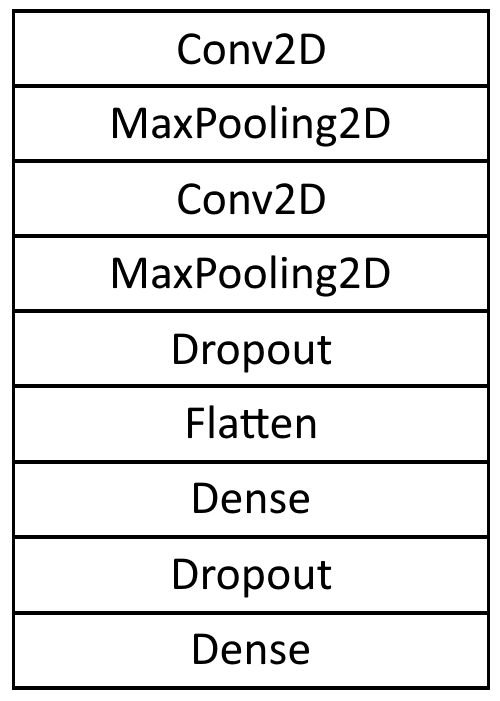
\includegraphics[width=35mm]{images/healthy_model.png}
\caption{CNN classifying patient's healthiness and the type of glioma}
\label{fig:simple_cnn_model}
\end{wrapfigure}
Surprisingly the network was always able to reach 100~\% accuracy on the validation set after one epoch of training with about two third of the provided data.
It was easy to train on the provided data because healthy and unhealthy images had some magnificent differences. \\
In our first approach the images containing a tumor had no skull and were brighter than the healthy image.
The second dataset was augmented so the unhealthy images also contained a skull.
Unfortunately, one could clearly see the difference between augmented and real brain scans.
Examples of the first and second datasets for healthy and unhealthy patients are shown in Figure \ref{fig:healthy_samples}.
Again it was very easy for the network to converge.
After scaling the images to a low resolution the calculations were very fast and initially produced better accuracy before converging to the optimum.

\begin{figure}[t]
\begin{center}
\includegraphics*[width=0.7\textwidth]{images/healthy_unhealthy_samples_mixed.png}\\
\caption{(1) Comparison of four patients, two of whom suffering from a tumor. Notice the different brightness and the missing skull on the scans of the unhealthy patients.\\
(2) The unhealthy labeled scans from row (1) are augmented so they contain a skull. The difference in brightness still remains.}
\label{fig:healthy_samples}
\end{center}
\end{figure}


\subsection{Low-Grade Glioma vs. High-Grade Glioma}

For the treatment of the tumor and the patient's survival rate it's important to know which type of tumor the patient is suffering from.
As pointed out by Menze et al. \cite{journals/tmi/MenzeJBKFKBPSWL15} in their paper related to the BraTS challenge the life expectancy highly varies depending on the type of glioma.
Usually patients will survive several years if they're suffering from a LGG.
In contrast to this, patients with the more aggressive HGG have a median survival rate of two years or less. \\
For this task we were looking at the ground truth dataset for task one which solely consists of images of the tumor itself instead of the whole brain.
Again as in the previous classification task there were only two classes and the network received a similar input shape.
That's why we decided to apply the same model on this task.
The network was trained on another dataset containing 25.000 tumor images and again converged very quickly with about 95~\% accuracy as you can see in Figure \ref{fig:hgg_lgg_history}.

\begin{figure}[hbp]
\begin{center}
\includegraphics*[width=0.7\textwidth]{images/hgg_lgg_history.png}\\
\caption{Using a very similar network as in the previous classification task we got a high accuracy on classifying HGG and LGG.}
\label{fig:hgg_lgg_history}
\end{center}
\end{figure}


\section{Tumor Segmentation}
\label{sec:segmentation}
\subsection{Conditional Adversarial Networks}
As we already stated in Section \ref{sec:classification}, having too few data is a giant problem when trying to apply Deep Learning algorithms.
Even when trying to artificially extend the available data by e.g. adding tumors to known positions of healthy scans, it is easy to introduce properties to the images that make it easier for the applied algorithms to find those artificial tumors than real tumors.
To solve this problem, we used a Conditional Generative Adversarial Network (cGAN) for the tumor segmentation, which is a special kind of Generative Adversarial Network.

Generative Adversarial Networks (GANs) have been introduced by Goodfellow et al.\cite{GANs}.
They learn to artificially create objects that highly resemble samples of a given real dataset.
A simplified depiction of a GAN can be found in Figure \ref{fig:gan}.
\begin{figure}[hbp]
\begin{center}
\includegraphics*[width=0.7\textwidth]{images/generative-adversarial-network.png}\\
\caption{A GAN that learns to generate fake samples that can hardly be distinguished from real samples (from \cite{KDnuggets_GAN})}
\label{fig:gan}
\end{center}
\end{figure}

They consist of two agents: a discriminator and a generator.
The generator receives a vector containing random noise as input and generates an output.
The discriminator receives this output of the generator and a sample of the real dataset and decides, whether the given input is real or fake, meaning its origin is the dataset or the generator, respectively.
The discriminator receives feedback whether its guess was right or wrong.
The generator in turn receives feedback whether he was able to "fool" the discriminator, meaning the generated object resembled the samples of the real dataset so well that the discriminator was not able to distinguish between them.

Conditional Generative Adversarial Networks cGANs have been introduced by Isola et al.\cite{cGANs}.
\begin{figure}[ht]
\begin{center}
\includegraphics*[width=0.95\textwidth]{images/conditional-adversarial-network.png}\\
\caption{Isola et al. show that cGANs are very well suited for image-to-image translations like colorizing black and white pictures or transforming day pictures to night pictures.}
\label{fig:can}
\end{center}
\end{figure}

The real dataset of cGANs consists of picture tuples of an input and an output image.
Additionally to random noise, generator of a cGAN also receives the input image and is supposed to generate an output image that is accepted by the discriminator.
The discriminator, on the other hand, learns to decide whether an output image fits to the given input image or not.
Thus, the generator is more restricted to the mapping he is supposed to learn.
Isola et al. were able to show that this creates very promising results even with very complex graphical structures.

\subsection{Network Architecture}

% This section is about the pix2pix model and changes that improved our result
Our segmentation network is based on pix2pix\footnote{\url{https://github.com/yenchenlin/pix2pix-tensorflow}}, which is a cGAN.
This model uses U-Net \cite{DBLP:journals/corr/RonnebergerFB15} for the generator and a Markovian Discriminator \cite{cGANs}.
The network produces good results with generative tasks.
Our contribution is to test the applicability for medical image segmentation.
To achieve this it was necessary to refactor the implementation, albeit the model structure was not changed.\\
The most important change was made regarding the used data.
The original implementation used a RGB image as an input and predicted a RGB image as well.
A first test with this model produced very bad results (Figure \ref{fig:demo_input}).
The reason for this is mainly restrictions regarding the input and the output of the model.
It only supports one image for both, but to get good results we need all four modalities (Figure \ref{fig:demo_input}).
However the biggest improvement was to split the ground truth into three different label masks.
Each mask encodes only one label.
This eliminates the gradients between different labels in one image.
To retrieve the actual output it is required to merge the different label masks again.\\
To improve the model performance we use gray-scale images instead of RGB images.
This reduces the memory consumption to a level that is comparable with the original implementation.
This leaves room for further expansion of the used model.
To improve the generator we doubled the depth of each convolutions and also increased the size of each convolution from 5x5 to 6x6.
Both changes increased the accuracy at the cost of a much longer training time.\\
Another way to improve the result is by using smart data selection.
Instead of training the model with images from every axis, we only use one axis.
This increases the result for one axis drastically, because each axis contains a different set of features.
Also the size of the images is not uniform for all axes.
To reduce the training time we additionally implemented virtual batch normalization \cite{DBLP:journals/corr/SalimansGZCRC16}.
To achieve a faster training process, we ordered the data, so that each batch only consisted of similar images.

\section{Survival Rate Prediction}
\label{sec:survival}
The consecutive second task of the BraTS challenge was to use the segmented tumor of the patient to predict the patient's overall survival rate.
The only additional feature that was given was the patient's age.
The label was a number between zero and 1750 which represented the number of days the patient lived after the scans where taken.
Thus, this task might have been even more challenging than the first one because the information-to-noise ratio was even worse as the target label was only a single number for a whole 3D brain scan that included segmented tumors.
Additionally, any wrong segmentation that was made during task one would also influence this tasks prediction.\\
To artificially create more training data, we considered using data augmentation.
Though, while we're no experts in the field of neuroscience, we had to assume that the size and location of a tumor highly influences the patient's survival rate.
Thus, we rejected using data augmentation by scaling, rotating or moving the segmented tumors as it could have falsified the survival rate, introducing even more noise into the dataset. \\

For evaluating the importance of the patient's age we looked at the correlation of the age and the survival rate. As you can see in in Figure \ref{fig:sr_vs_age} the survival rate slightly decreases with an increasing age of the patient.

\begin{figure}[hbp]
\begin{center}
\includegraphics*[width=0.75\textwidth]{images/Survival_vs_Age.png}\\
\caption{The survival rate of a patient decreases with an higher age of the patient. The datapoints are widely spread so we have a weak correlation. The Pearson's correlation coefficient overall 163 datapoints is about $-0.37$ . }
\label{fig:sr_vs_age}
\end{center}
\end{figure}

To predict the survival rate of a patient, one team member tried to use classical machine learning models while another one used a convolutional neural network approach.
The information regarding brain and tumor of a patient was given as seven 3D images.
Three of them were representing the tumor regions while the remaining four were the input for task one showing the brain using different modalities.
Each 3D model had a shape of 120 Pixels x 120 Pixels x 129 Slices.
To break down the tumor segments to comparable variables, we did some analysis and extracted values like the size of the tumor:

\begin{itemize}
\item \textbf{TumorSum1}: All pixels labeled as part of the first tumor region
\item \textbf{TumorSum2}: All pixels labeled as part of the second tumor region
\item \textbf{TumorSum3}: All pixels labeled as part of the third tumor region
\item \textbf{TumorSum}: Sum of the previous three values
\item \textbf{BrainSum}: All pixels labeled as part of the brain
\end{itemize}

We used the sum of pixels to represent the size of a 3D object.
Because all images had the same resolution, it would have ended up in scaling the values by the same factor so the correlation matrix would look the same.

\begin{figure}[hbp]
\begin{center}
\includegraphics*[width=0.75\textwidth]{images/corr_matrix_numbers.png}\\
\caption{The correlation between all extracted numerical values regarding the second task. Note that the size of a brain decreases with the patient's age as well as the patient's survival rate.}
\label{fig:corr_matrix}
\end{center}
\end{figure}

Figure \ref{fig:corr_matrix} shows the correlation matrix for the patient's age, the survival rate and the other five previous mentioned variables.
Although the correlation between age and survival rate seemed to be very weak regarding Figure \ref{fig:sr_vs_age} it is the strongest one among all the other variables in comparison with the survival rate. \\

\subsection{Using Support Vector Regression}


Using the Python library scikit-learn\cite{scikit-learn}, we collected all regression models (Bayesian Ridge Regression, Stochastic Gradient Descent Regressor, Support Vector Regression etc.) and cross-validated them on the aforementioned features of the training data.

The Support Vector Regression (SVR) clearly outperformed the remaining regression approaches.
To fine tune the model, we tried different kernels that are mapped on the data before the regression function is fit to the data.
In Figure\ref{fig:svr_kernels} one can see that the SVR with the lowest mean squared error (MSR) basically just learned to predict the average of the survival rate distribution.
This is a strong indicator that the approach is still in the early stages of development.


\begin{figure}[!t]
\begin{center}
\includegraphics*[width=0.9\textwidth]{images/svr_kernels.png}\\
\caption{We varied the kernels that were applied to the data, namely a radial basis function, a sigmoid and a quadratic kernel (from left to right). The values for the MSR were 44.000, 43.000 and 39.000. It's worth noting that the smaller the error gets, the more often the related SVR predicts the average value of the survival day distribution.}
\label{fig:svr_kernels}
\end{center}
\end{figure}

\subsection{Using Convolutional Neural Networks}

In contrast to the approach of using Support Vector Regression we added the segmented tumor from task one. The image data provides information regarding the position and the size of the tumor which might influence the survival rate of the patient. \\

\subsubsection{Model}

As previously mentioned we assumed that the tumor's position might be important for the survival rate.
That's why we decided to use a CNN respecting the whole brain and the tumor instead of extracting usable information as done in our previous analysis. \\
Our network processing the different types of input data is shown in Figure \ref{fig:sr_network}.
To merge the multi-input including different data types we used a CNN which is combined with the patients age via a concatenation layer.
In the end we applied some final dense layers ending up in a number representing the survival rate of the patient. \\

The age of patient is a number within the interval from 0 to 100.
Because we expect a non linear behavior regarding the survival rate we wanted to transform the age into classes.
This way each class can influence the whole regression task in another way and the input is limited to a certain range of classes.
The transformation is done by applying one-hot encoding which is a usual procedure in the field of machine learning to transform some values into classes.

\begin{figure}[hbp]
\begin{center}
\includegraphics*[width=0.75\textwidth]{images/sr_model.png}\\
\caption{Rough structure of the network receiving a patient's age and images regarding his tumor and his whole brain.
It's based on the concatenation network from the Keras documentation \textsuperscript{3}.
The main output is a float number between zero and one which gets scaled up to 2000.}
\vspace*{5mm}\small\textsuperscript{3} \url{https://keras.io/getting-started/functional-api-guide/#multi-input-and-multi-output-models}
\label{fig:sr_network}
\end{center}
\end{figure}

\subsubsection{Results}

Because we're missing the most important part for our work, which is a lot of data, our network didn't converge to any reasonable results.
We tried out different optimizer, decreased the dropout rate, reduced the input size in different ways and applied many other changes on our network structure, but unfortunately we couldn't fix this problem. \\
One of our attempts included transforming the 3D models into 2D images.
Instead of considering the three-dimensional arrangement within the brain we look at a cross sectional area.
This cross-section image visualized the density of a two-dimensional point over the whole third dimension. An example for the output of this transformation is shown in Figure \ref{fig:tumor_2d}. \\

\begin{figure}[!h]
\begin{center}
\includegraphics*[width=0.75\textwidth]{images/tumor_2d.png}\\
\caption{Outcome of the transformation from 3D to 2D images for three tumor regions and one of the four given brain modalities.}
\label{fig:tumor_2d}
\end{center}
\end{figure}

\section{Demo Tool}
\label{sec:demo}
Based on our model that has been developed in Section \ref{sec:segmentation}, we built an interactive demo tool.
As an input, it takes a PNG image file consisting of the FLAIR, T1, T1CE and T2 scans of a patient's brain slice.
For this example we consider as input the picture depicted in Figure \ref{fig:demo_input}.
The server needs a few seconds to compute the predicted tumor classes, given there are any.
The output image can be seen in Figure \ref{fig:demo_output}.
The tool highlights the necrotic and non-enhancing tumor in blue, the GD-enhancing tumor in red and the peritumoral edema in yellow.
In this example, the server recognized the tumor as a HGG. \\
For the direct usage of our trained networks we've set up a python server which receives the images of a patient and returns the results of our networks.
Our frontend application is based on JavaScript using Redux and React.

\begin{figure}[!h]
\begin{center}
\includegraphics*[width=0.6\textwidth]{images/demo_output.png}\\
\caption{Demo tool with segmented tumor and classified tumor type based on input image from Figure \ref{fig:demo_input}}
\label{fig:demo_output}
\end{center}
\end{figure}

\newpage

\section{Conclusion and Future Work}
\label{sec:conclusion}

This section contains a conclusion for both BraTS challenges.

\subsection{Segmentation}

The segmentation model we proposed is successfully predicting tumor positions.
We definitely improved the approach we worked on as one can see in Figure \ref{fig:demo_input} (3).
However, our prediction is still far away from being perfect which has multiple reasons.
First of all we only use two-dimensional images and do not combine features of neighbouring images.
This leads to missing very small tumors and sometimes predicting very small, false  tumors at random locations.
One possibility to solve this problem is by using the three-dimensional information that is present in the data.
Missing small tumors decreased our rank in the BraTS challenge a lot because for each patient the accuracy was averaged.
We usually achieved accuracies above 90\% but the false positive detections were calculated as 0\% and impaired our final rank.\\
While working on our model we found some additional flaws in it.
The biggest mistake is probably the choice of the loss function.
We use multiple masks with sigmoid-cross-entropy but every other segmentation model uses a softmax layer with categorical-cross-entropy.
Our approach has the drawback that we needed to merge the three tumor masks we predicted in order to submit our result.
A problem with this operation is that there is no good way of merging overlapping masks.
Having one softmax layer for each pixel would solve this problem because we would only generate one label per pixel.
This would also solve the problem that we do not scale well for many different segmentation classes.\\
Another problem is that our mask method requires post-processing to generate the output.
Due to not using softmax we always generate images that contain gradients between -1 and 1 which have to be mapped to binary values using the sigmoid function.
The three binary masks then have to be merged into one image.\\
Due to the use of U-Nets our model has lots of parameters so we need a long training time (basically two weeks on two Titan X GPUs). The segmentation performance is about one fps.\\
To keep the U-Net encoder/decoder simple we also had to always use images with dimensions of a power of two.
Since the shapes of the images of the BraTS data are not a power of two, we always had to pad the scans.
The perceived flaws are leaving enough space for further improvements.

\subsection{Segmentation Improvements}

One way to improve the results is to use a refinement network to post-process to generated predictions.
This network could use the sequence property of the used medical data.
To use this additional information it is possible to use a U-Net that utilizes a LSTM node to process the encoded input.
This model should learn a different set of features than the first one.
In order to achieve this we would not train on the ground truth.
Instead we would train using the error of the original prediction.
The model then learns an error function that can be used to further improve our results.\\
The LSTM idea can also be directly implemented into the cGAN.
This way the generator and discriminator themselves are aware of the sequence property.
A problem with this approach is that it reduces the amount of input data from 285x155 images to 285 sequences, which increases the problem of overfitting.

\subsection{Survival Rate Prediction}
While we can detect the presence and the type of a brain tumor and also received good results in segmenting the tumor region, we were not able to predict the patient's survival rate in a satisfying matter.
In comparison to the other tasks we couldn't augment data to create a bigger training dataset.
Furthermore, it included a more complex relation between input and output.
We inspected the correlations between the received data and the ground truth labels to get a better understanding of the correlations.
Unfortunately our assumptions were not precise enough to successfully train a network on the dataset.
The survival rate might depend on several other factors than the patient's age so it would be helpful to have more medical research on this topic to improve the dataset. \\


\newpage
%%%% bibtex file %%%%%%
%\bibliographystyle{alphadin}
\bibliographystyle{ieeetr}
\bibliography{references}

\end{document}
